\documentclass[10.5pt,a4paper]{article}
\usepackage[utf8]{inputenc}
\usepackage[T1]{fontenc}
\usepackage{lmodern}
\usepackage[margin=1.8cm]{geometry}
\usepackage{amsmath,amssymb}
\usepackage{booktabs,longtable,array,tabularx}
\usepackage{xcolor}
\usepackage{graphicx}
\usepackage[hidelinks]{hyperref}
\usepackage{fancyhdr}

\definecolor{accent}{HTML}{1F4E79}
\definecolor{soft}{HTML}{EAF1F8}
\definecolor{warn}{HTML}{FFF4E0}
\definecolor{warnline}{HTML}{C77700}

\makeatletter
\renewcommand\section{\@startsection{section}{1}{0pt}{1.3em plus .3em minus .2em}{0.4em}{\Large\bfseries\color{accent}}}
\renewcommand\subsection{\@startsection{subsection}{2}{0pt}{1.0em plus .2em minus .1em}{0.3em}{\large\bfseries\color{accent}}}
\makeatother
\setlength{\parindent}{0pt}
\setlength{\parskip}{0.4em}
\renewcommand{\arraystretch}{1.22}
\let\olditemize\itemize\renewcommand\itemize{\olditemize\setlength\itemsep{0.1em}\setlength\topsep{0.25em}}
\let\oldenumerate\enumerate\renewcommand\enumerate{\oldenumerate\setlength\itemsep{0.1em}\setlength\topsep{0.25em}}
\pagestyle{fancy}\fancyhf{}
\fancyhead[L]{\small q6 re-analysis and half-the-box check}\fancyhead[R]{\small page \thepage}
\renewcommand{\headrulewidth}{0.3pt}
\newsavebox{\mybox}
\newenvironment{keybox}{\par\medskip\noindent\begin{lrbox}{\mybox}\begin{minipage}{\dimexpr\linewidth-2\fboxsep-2\fboxrule\relax}}{\end{minipage}\end{lrbox}\noindent\fcolorbox{accent}{soft}{\usebox{\mybox}}\par\medskip}
\newenvironment{warnbox}{\par\medskip\noindent\begin{lrbox}{\mybox}\begin{minipage}{\dimexpr\linewidth-2\fboxsep-2\fboxrule\relax}}{\end{minipage}\end{lrbox}\noindent\fcolorbox{warnline}{warn}{\usebox{\mybox}}\par\medskip}

\newcommand{\ps}{p^{*}}
\begin{document}
\begin{center}
{\LARGE\bfseries\color{accent} q6 re-analysis and the half-the-box check\\[2pt]}
{\large Existing trajectories only, no new simulations}
\end{center}

\begin{keybox}
\textbf{Results in five lines.}
(1) The ref.\ [18] thresholds (0.5, cutoff 1.5) are \textbf{not usable as they are} here: they call about 54 of 1000 particles solid-like in the starting liquid, but the paper says fewer than 5. Your stricter settings (0.70, cutoff 1.45) give about 1, which fits the paper.
(2) In the dr $=0.04$ run the crystal \textbf{wraps through the periodic box} from about $2.1$--$2.15\times10^{6}$ cycles on, so the plateau near 500 (PTM) is a \textbf{finite-size limit}, not a nucleus size.
(3) By q6 (your settings) the crystalline region is about \textbf{800 of 1000} particles at the end; PTM counts only 486 as fcc/hcp.
(4) Charge order in the crystal is \textbf{not higher than in the liquid} (0.58 vs.\ 0.60 opposite-charge neighbours), consistent with a substitutionally disordered crystal.
(5) The June cluster of 70 is \textbf{not a crystal by PTM} (at most 16 crystalline particles in those frames).
\end{keybox}

\section{What was done}
\begin{itemize}
\item \texttt{q6\_fast.py}: a vectorised copy of your \texttt{analyze\_q6\_cluster.py} with a switch for the cluster-joining rule. \textbf{Validation:} it reproduces your original \texttt{cluster\_size.dat} exactly on 101 frames of the June run (0 mismatches), including the peak region.
\item Two settings on \textbf{every saved frame}: \emph{ref18} (cutoff 1.5, dot $>0.5$, $\ge7$ connections, join any neighbouring solid-like particles) and \emph{yours} (1.45, $>0.70$, $\ge7$, join only through connected bonds). Data: dr $=0.04$ and dr $=0.01$ campaigns (3001 frames each) and the June run (2001 frames).
\item Half-the-box check on six dr $=0.04$ frames: OVITO PTM (RMSD 0.10), largest cluster with unwrapped coordinates (extent along x, y, z and whether it connects to its own periodic image), and the fraction of opposite-charge nearest neighbours.
\end{itemize}
Everything is in \texttt{zNotes/q6\_check/} (scripts, CSV per trajectory, plot). Your run folders and original scripts were not touched.

\section{The ref.\ [18] thresholds do not work for this liquid}
Mean number of particles called solid-like and largest cluster in the first $5\times10^{4}$ cycles (all PTM-validated liquid, paper: fewer than 5 of 1000):

\begin{center}\small
\begin{tabular}{@{}lcccc@{}}
\toprule
 & \multicolumn{2}{c}{ref.\ [18] settings} & \multicolumn{2}{c}{your settings}\\
Trajectory & solid-like & largest & solid-like & largest\\
\midrule
dr $=0.04$ campaign & 54 & 17 & 1.5 & $\le3$\\
dr $=0.01$ campaign & 53 & 14 & 0.7 & $\le2$\\
June run & 71 & 24 & 1.2 & $\le4$\\
\bottomrule
\end{tabular}
\end{center}
The thresholds of ref.\ [18] were fixed for Lennard-Jones at fcc--liquid coexistence. In this dense binary hard-core Yukawa liquid they produce about 5\% false solid-like particles. \textbf{So my earlier recommendation (use 0.5 as the baseline) was wrong for this system; the recommendation is corrected in the Task 2 note.} Your stricter 0.70 reproduces the paper's own liquid calibration, which suggests the authors also used tighter thresholds than ref.\ [18] (not stated in the paper).

\begin{figure}[h]\centering
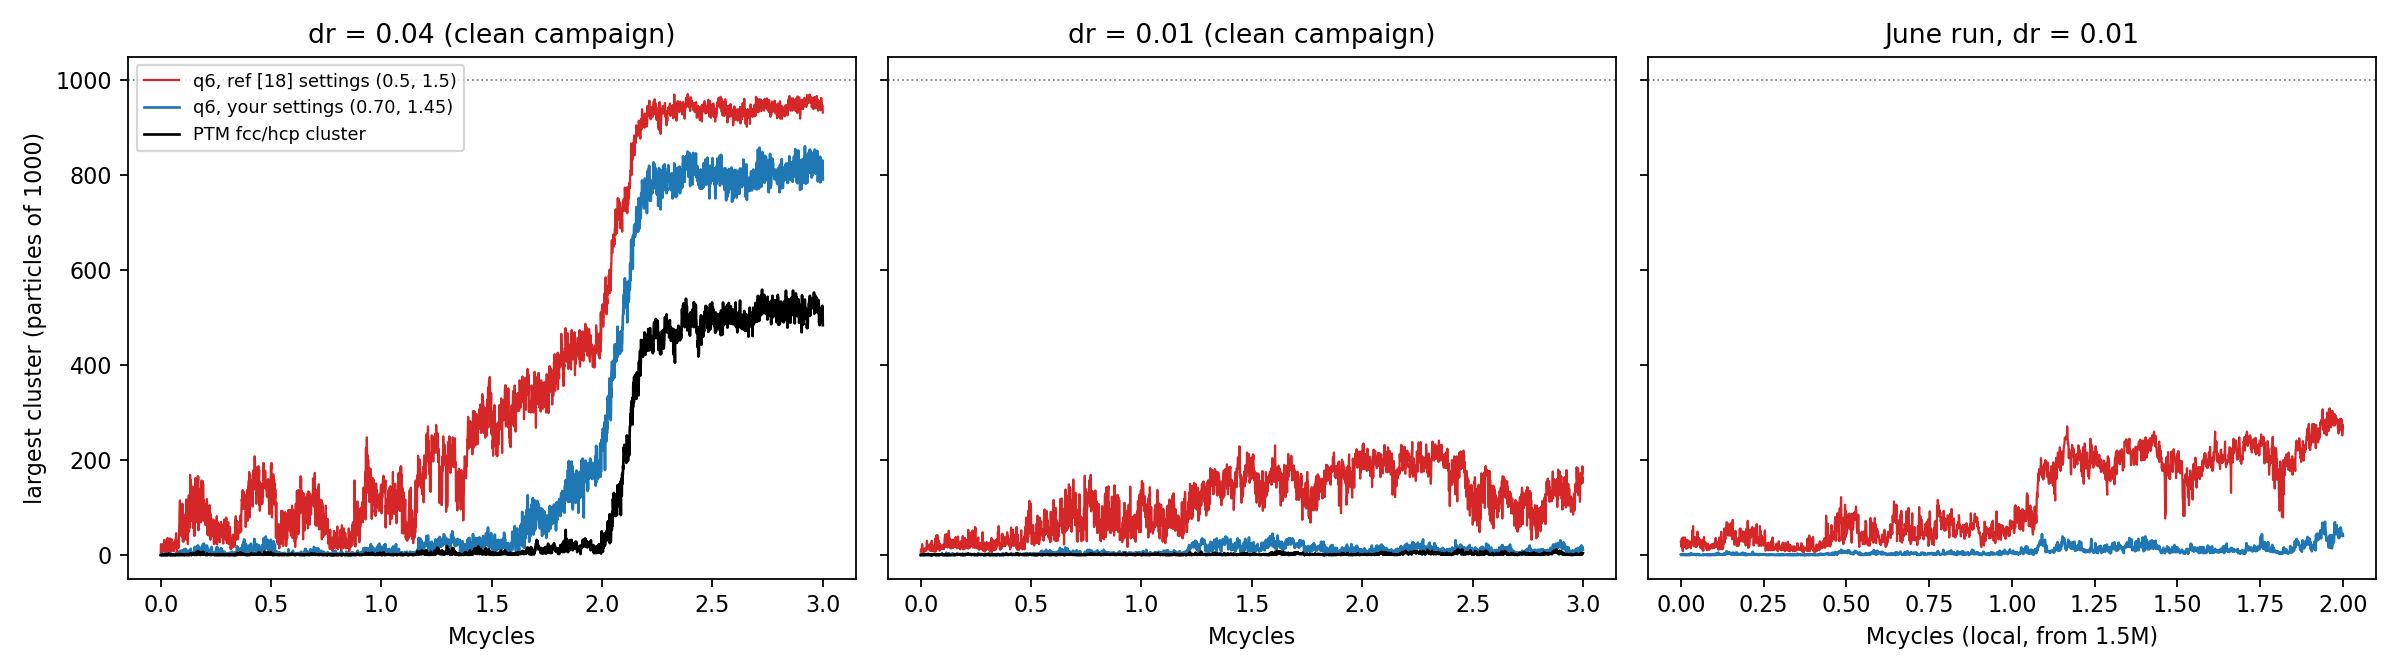
\includegraphics[width=\textwidth]{figs/q6_vs_ptm.png}
\caption{Largest cluster per frame. Red: ref.\ [18] settings (inflated by liquid false positives). Blue: your settings. Black: PTM fcc/hcp cluster. Dashed line: all 1000 particles.}
\end{figure}

\section{Half-the-box check (dr $=0.04$)}
Extent is measured along x/y/z with unwrapped coordinates; the box edge is about 9.7--9.8$\sigma$. ``wrap'' lists the directions in which the cluster connects to its own periodic image.

\begin{center}\small
\begin{tabular}{@{}lccc@{}}
\toprule
Cycles & PTM crystal cluster & q6 (yours) cluster & PTM fcc / hcp / bcc\\
\midrule
2.00M & 24, no wrap & 237, wraps x z & 13 / 18 / 4\\
2.05M & 109, no wrap & 410, wraps x y z & 46 / 62 / 7\\
2.10M & 224, wraps x z & 526, wraps x y z & 93 / 127 / 7\\
2.15M & 364, wraps x y z & 682, wraps x y z & 124 / 246 / 2\\
2.25M & 483, wraps x y z & 761, wraps x y z & 146 / 337 / 0\\
3.00M & 486, wraps x y z & 791, wraps x y z & 160 / 324 / 2\\
\bottomrule
\end{tabular}
\end{center}
\textbf{Reading.}
\begin{itemize}
\item From about 2.15M cycles the PTM cluster is connected to its own periodic images in all three directions. It cannot grow as an isolated droplet any more, so the plateau near 500 is set by the box, not by the physics. \textbf{Quote the nucleation time, not the final size.}
\item The two measures disagree on how much is crystalline (486 vs.\ about 790). PTM with a strict RMSD cutoff probably rejects thermally distorted crystal as ``other'', and q6 counts distorted and defective regions; I cannot tell from this data which is closer to the truth, so give both.
\item Already at 2.0M cycles q6 shows a region of 237 particles that wraps in x and z, while PTM sees 24. Between 1.5M and 2.0M the q6 cluster grows steadily (mean 110, maximum 243) before the PTM jump. This is either a real precursor of the crystal or ordered liquid that q6 over-counts; the data do not decide.
\item Critical-nucleus size (about 120 at $\ps=15$ in the paper) cannot be read off these runs: the nucleus is already wrapped by the time it is larger than a few hundred particles.
\end{itemize}

\subsection*{Charge order in the crystal}
Fraction of nearest-neighbour pairs (distance $<1.3\sigma$) with opposite charge, among PTM fcc/hcp particles of the cluster: \textbf{0.58} at 2.1M--3.0M cycles. The starting liquid gives \textbf{0.60}; random mixing would give 0.50. An ordered arrangement (for example CuAu-type) would give about 0.67 or more. So the crystal has \emph{no extra} charge order compared with the liquid: consistent with substitutional disorder, as in the paper. (Limits: only fcc/hcp-labelled particles, and the 1.3$\sigma$ cutoff is my choice.)

\section{The June run}
The June cluster of 70 (your settings, around $1.95\times10^{6}$ cycles into that run) is \textbf{not confirmed as a crystal}: PTM finds at most 6 fcc, 10 hcp and 1 bcc in those frames.

\begin{center}\small
\begin{tabular}{@{}lcccccc@{}}
\toprule
Local cycle & 0 & 1.0M & 1.5M & 1.946M & 1.976M & 2.0M\\
\midrule
PTM fcc + hcp + bcc & 0 & 2 & 7 & 12 & 16 & 7\\
\bottomrule
\end{tabular}
\end{center}
With the ref.\ [18] settings the same run shows 309, which again illustrates that those thresholds over-count. Your original decision to distrust that cluster is supported.

\section{What is still open}
\begin{itemize}
\item Which of PTM (486) and q6 (about 790) is closer to the real crystalline fraction. A visual check in OVITO (type colouring, Replicate $2\times2\times2$, PTM at RMSD 0.10 and 0.15) is the natural next step.
\item Whether the q6 precursor between 1.5M and 2.0M is real. Frames of \texttt{seg008}--\texttt{seg009} are the place to look.
\item A larger system (for example $N=2000$) would be needed to measure an isolated nucleus; that is a new simulation and has not been started.
\item Re-tune the q6 thresholds against the paper's liquid calibration (fewer than 5 solid-like of 1000), for example scanning dot $\in[0.5,0.8]$.
\end{itemize}
\end{document}
